\documentclass[a4paper, 11pt]{report}
\usepackage[utf8]{inputenc} % Required for inserting images
\usepackage{graphicx}
\usepackage[hidelinks]{hyperref}
\usepackage{blindtext}
\usepackage[T1]{charter}
\usepackage{caption}
\usepackage[
backend=biber,
style=alphabetic,
sorting=ynt
]{biblatex}
\addbibresource{sample.bib}
{\fontfamily{bch}\selectfont
\title{SPM}
\author{Parth Sonani}
\date{November 2023}

\begin{document}
\begin{titlepage} % Suppresses displaying the page number on the title page and the subsequent page counts as page 1
	\newcommand{\HRule}{\rule{\linewidth}{0.5mm}} % Defines a new command for horizontal lines, change thickness here
	
	\center % Centre everything on the page
	
	%------------------------------------------------
	%	Headings
	%------------------------------------------------
	
	\textsc{\LARGE Concordia University}\\[1.5cm] % Main heading such as the name of your university/college
	

	%------------------------------------------------
	%	Title
	%------------------------------------------------
	
	\HRule\\[0.4cm]
	
	{\huge\bfseries  SOEN 6841 - Software Project Management}\\[0.4cm] % Title of your document
	
	\HRule\\[1.5cm]
	\textsc{\Large Topic Analysis and Synthesis}\\[0.5cm] % Major heading such as course name
	\textsc{\Large Continuous Kindness}\\[0.5cm]
	%------------------------------------------------
	%	Author(s)
	%------------------------------------------------
	
			\large
			\textit{Supervisor}\\
			Prof. Pankaj Kamthan\\[0.5cm] % Supervisor's name
% 		\end{flushright}
% 	\end{minipage}
    \vfill
    \large
			\textit{Author}\\
            Parth Sonani - \textsc{40221824}\\
            
	
	\vfill\vfill\vfill\vfill% Position the date 3/4 down the remaining page
	\textbf{GitHub Address:} \url{https://github.com/ParthSonani/SOEN6841-TAS}

	%------------------------------------------------
	%	Logo
	%------------------------------------------------
	
 	\vfill\vfill
 	
\includegraphics[scale=0.5]{Concordia-logo.jpeg}\\[1cm] % Include a department/university logo - this will require the graphicx package
	 
	%----------------------------------------------------------------------------------------
	
	\vfill % Push the date up 1/4 of the remaining page
	
\end{titlepage}

\tableofcontents

\pagebreak

\section{Abstract}

In workplaces, working well together seems easy when we chat, work on projects, or have quick talks by the water cooler. But, in reality, it's not that simple. Despite knowing the basics like daily meetings and friendly banter, many workplaces face problems like too much work, confusing procedures, and tools that don't solve everything. Instead of focusing on what really matters—how people interact—many workplaces get distracted by new tools and trendy methods. The question is, why do we choose flashy technology over building better relationships? This story shifts the focus to something crucial: "kindness." It points out that a lack of kindness and related behaviors—like understanding, trust, and empathy—is what holds us back in workplace interactions. When we don't trust others, we add more rules instead of fixing relationships. We assume people don't get us, instead of explaining our issues. We get defensive instead of trying to understand why someone is upset. Breaking these habits isn't easy. It needs effort to be kind in all situations, to step back, and ask what's really going on. Being patient and understanding can be powerful. It builds trust and creates a positive environment, making work flow smoothly. And, being kind tends to spread—it influences others to approach situations constructively, making interactions better. Being tough might work for a while, but being kind goes much further—for you and everyone around you. It's not just about being nice; it's about creating a workplace where people get along, work well together, and everyone benefits.

\pagebreak
\section{Introduction}

In today's fast-paced workplaces, where achieving success is closely tied to how people interact, the concept of "Continuous Kindness" emerges as a guiding principle for fostering a positive organizational culture. Driven by the increasing understanding that an organization's triumph is intricately connected to the well-being of its workforce, there's a growing momentum to prioritize and embed kindness into the daily fabric of professional life. This goes beyond occasional acts of goodwill; it's a commitment to infuse daily work interactions with empathy, support, and positivity.
\vspace{5mm} %5mm vertical space
\newline
The motivation to explore the realm of continuous kindness is rooted in a substantial foundation of research and practical insights. A comprehensive systematic review conducted by David A. Fryburg (2023), titled "Kindness isn't just about being nice," sheds light on various strategies employed to instill kindness in professional settings [1]. This review not only highlights the multitude of benefits associated with workplace kindness but also acts as a catalyst for understanding the intricacies of implementing and sustaining kindness initiatives.
\vspace{5mm} %5mm vertical space 
\newline
Additionally, a thesis on "The impact of kindness in the workplace" (Deborah Lynn Kerr, 2008) contributes practical applications and real-world examples, emphasizing the adaptability and scalability of kindness initiatives [2]. Grounded in case studies, this resource provides a nuanced exploration of successful strategies and potential challenges, offering invaluable insights for organizations seeking to integrate kindness into their professional ethos.
\vspace{5mm} %5mm vertical space
\newline
These references collectively emphasize that continuous kindness is not just an idealistic pursuit; it's a strategic imperative for contemporary organizations. Workplaces are evolving, and so are the expectations of the workforce. Employees are now seeking environments where their overall well-being is valued, and organizations that embrace continuous kindness are better positioned to meet these expectations. This creates a symbiotic relationship between organizational success and employee fulfillment. In the following sections, we will delve into the identified problem statement, objectives, background materials, methods, results, and the potential implications of continuous kindness in the workplace.


\subsection{Motivation}

The motivation behind delving into the realm of continuous kindness stems from the growing acknowledgment that the success of an organization extends beyond financial metrics. Employee well-being, job satisfaction, and the quality of professional relationships significantly impact overall organizational performance. This section delves into the evolving expectations of the modern workforce, emphasizing the need for a workplace culture that prioritizes kindness as a catalyst for improved morale and sustained success.

\subsection{Problem Statement}
Despite the recognized benefits of fostering a culture of kindness, many workplaces face challenges in consistently implementing and maintaining such a culture. This report articulates the prevailing issues, ranging from high stress levels to strained interpersonal relationships, underscoring the need for intentional efforts to overcome these obstacles. The objective is to establish a foundation for understanding the existing gaps and formulating strategies to infuse kindness into the daily fabric of professional life.

\subsection{Objective}
The primary objective of this report is to investigate the feasibility and impact of integrating continuous kindness into the workplace culture. This involves understanding the barriers hindering the promotion of kindness, identifying strategies to overcome these challenges, and exploring the potential benefits for both individuals and organizations.



\section{Background Materials}

Extending the exploration into the concept of continuous kindness at the workplace, the following references have been instrumental in shaping the contextual understanding of this subject.
\vspace{5mm} %5mm vertical space
\newline
\noindent\textbf{Title: "Kindness Isn’t Just about Being Nice" [1]} 
\\
Link: \url{https://www.mdpi.com/2076-328X/13/6/457}
\begin{itemize}
    \item This systematic review delves into the existing body of research on promoting workplace kindness. 
    \item It provides valuable insights into the different approaches, interventions, and outcomes associated with cultivating kindness in professional settings.
    \item The findings of this review contribute significantly to understanding the multifaceted nature of kindness in the workplace.
\end{itemize}

\vspace{5mm} %5mm vertical space

\noindent\textbf{Title: "The Impact of Kindness in the Workplace" [2]}
\\
Link: \url{https://central.bac-lac.gc.ca/.item?id=MR55208&op=pdf&app=Library&is_thesis=1&oclc_number=738400260}
\begin{itemize}
    \item This thesis explores the practical aspects of fostering continuous kindness in organizational cultures.
    \item Drawing on case studies and real-world examples, it offers a detailed examination of successful strategies and potential challenges in implementing kindness initiatives.
    \item The thesis contributes to the development of practical frameworks for organizations aiming to instill kindness into their professional ethos.
\end{itemize}
\vspace{5mm} %5mm vertical space

These references provide a foundation for understanding the theoretical underpinnings and practical applications of continuous kindness in the workplace. Beyond these, a broader review of literature also reveals key themes such as the positive impact of kindness on employee engagement, the role of leadership in shaping a kind workplace culture, and the potential ripple effects of kindness on organizational performance.
\vspace{5mm} %5mm vertical space
\newline
Expanding upon the foundational literature, it is crucial to acknowledge the broader landscape of research on workplace dynamics. A study by Grant and Gino (2010) titled "A Little Thanks Goes a Long Way: Explaining Why Gratitude Expressions Motivate Prosocial Behavior"[5] underscores the positive impact of gratitude expressions on prosocial behavior. Drawing parallels between gratitude and kindness, this study contributes insights into the reciprocal nature of positive interactions and how expressions of appreciation can be integral to fostering a kind workplace culture.
\vspace{5mm} %5mm vertical space
\newline
Moreover, research by Dutton and Ragins (2007) in their work "Exploring Positive Relationships at Work: Building a Theoretical and Research Foundation"[6] delves into the significance of positive relationships in organizational settings. Their exploration of high-quality connections and the role of positive relationships in professional networks aligns with the broader theme of continuous kindness. Understanding the dynamics of positive connections at work is essential for organizations aiming to embed kindness as a consistent element in their culture.


\section{Methods and Methodology}
The mixed-methods approach adopted for this investigation involved qualitative interviews and case studies, as well as quantitative surveys. The interviews aimed to capture nuanced insights into existing workplace cultures, shedding light on the challenges faced and successful strategies employed in promoting continuous kindness. Case studies provided a deep dive into real-world scenarios, offering concrete examples of organizations that have successfully integrated kindness into their professional fabric.
\vspace{5mm} %5mm vertical space
\newline
Quantitative surveys were distributed across diverse industries to gather a broad spectrum of perspectives on the perceived impact of continuous kindness. The survey design incorporated validated scales to measure employee satisfaction, team collaboration, and organizational performance [7]. The triangulation of qualitative and quantitative data allowed for a comprehensive analysis, ensuring a well-rounded understanding of the feasibility and impact of fostering kindness in the workplace.
\vspace{5mm} %5mm vertical space
\newline
In addition to qualitative interviews and case studies, an analysis of social media sentiment related to workplace experiences was conducted. Leveraging natural language processing techniques, this approach provided a real-time glimpse into the online discourse surrounding workplace kindness. By mining sentiments expressed on platforms like Twitter and LinkedIn, it was possible to gauge the public perception of kindness initiatives in various organizations, offering an additional layer of insight into the external impact of internal cultural practices.


\section{Results}
The analysis of qualitative data revealed common themes, including the pivotal role of leadership in shaping a kind workplace, the significance of transparent communication, and the positive correlation between continuous kindness and employee well-being. Case studies illustrated the adaptability of kindness initiatives across various organizational structures, emphasizing the scalability and sustainability of such interventions.
\vspace{5mm} %5mm vertical space
\newline
Quantitative survey results affirmed the qualitative findings, indicating a positive association between perceived kindness in the workplace and heightened levels of job satisfaction. Furthermore, there was a noticeable correlation between workplace kindness and increased collaboration among team members. The results collectively highlight the potential for continuous kindness to serve as a catalyst for enhancing both individual and collective outcomes within organizational settings.
\vspace{5mm} %5mm vertical space
\newline
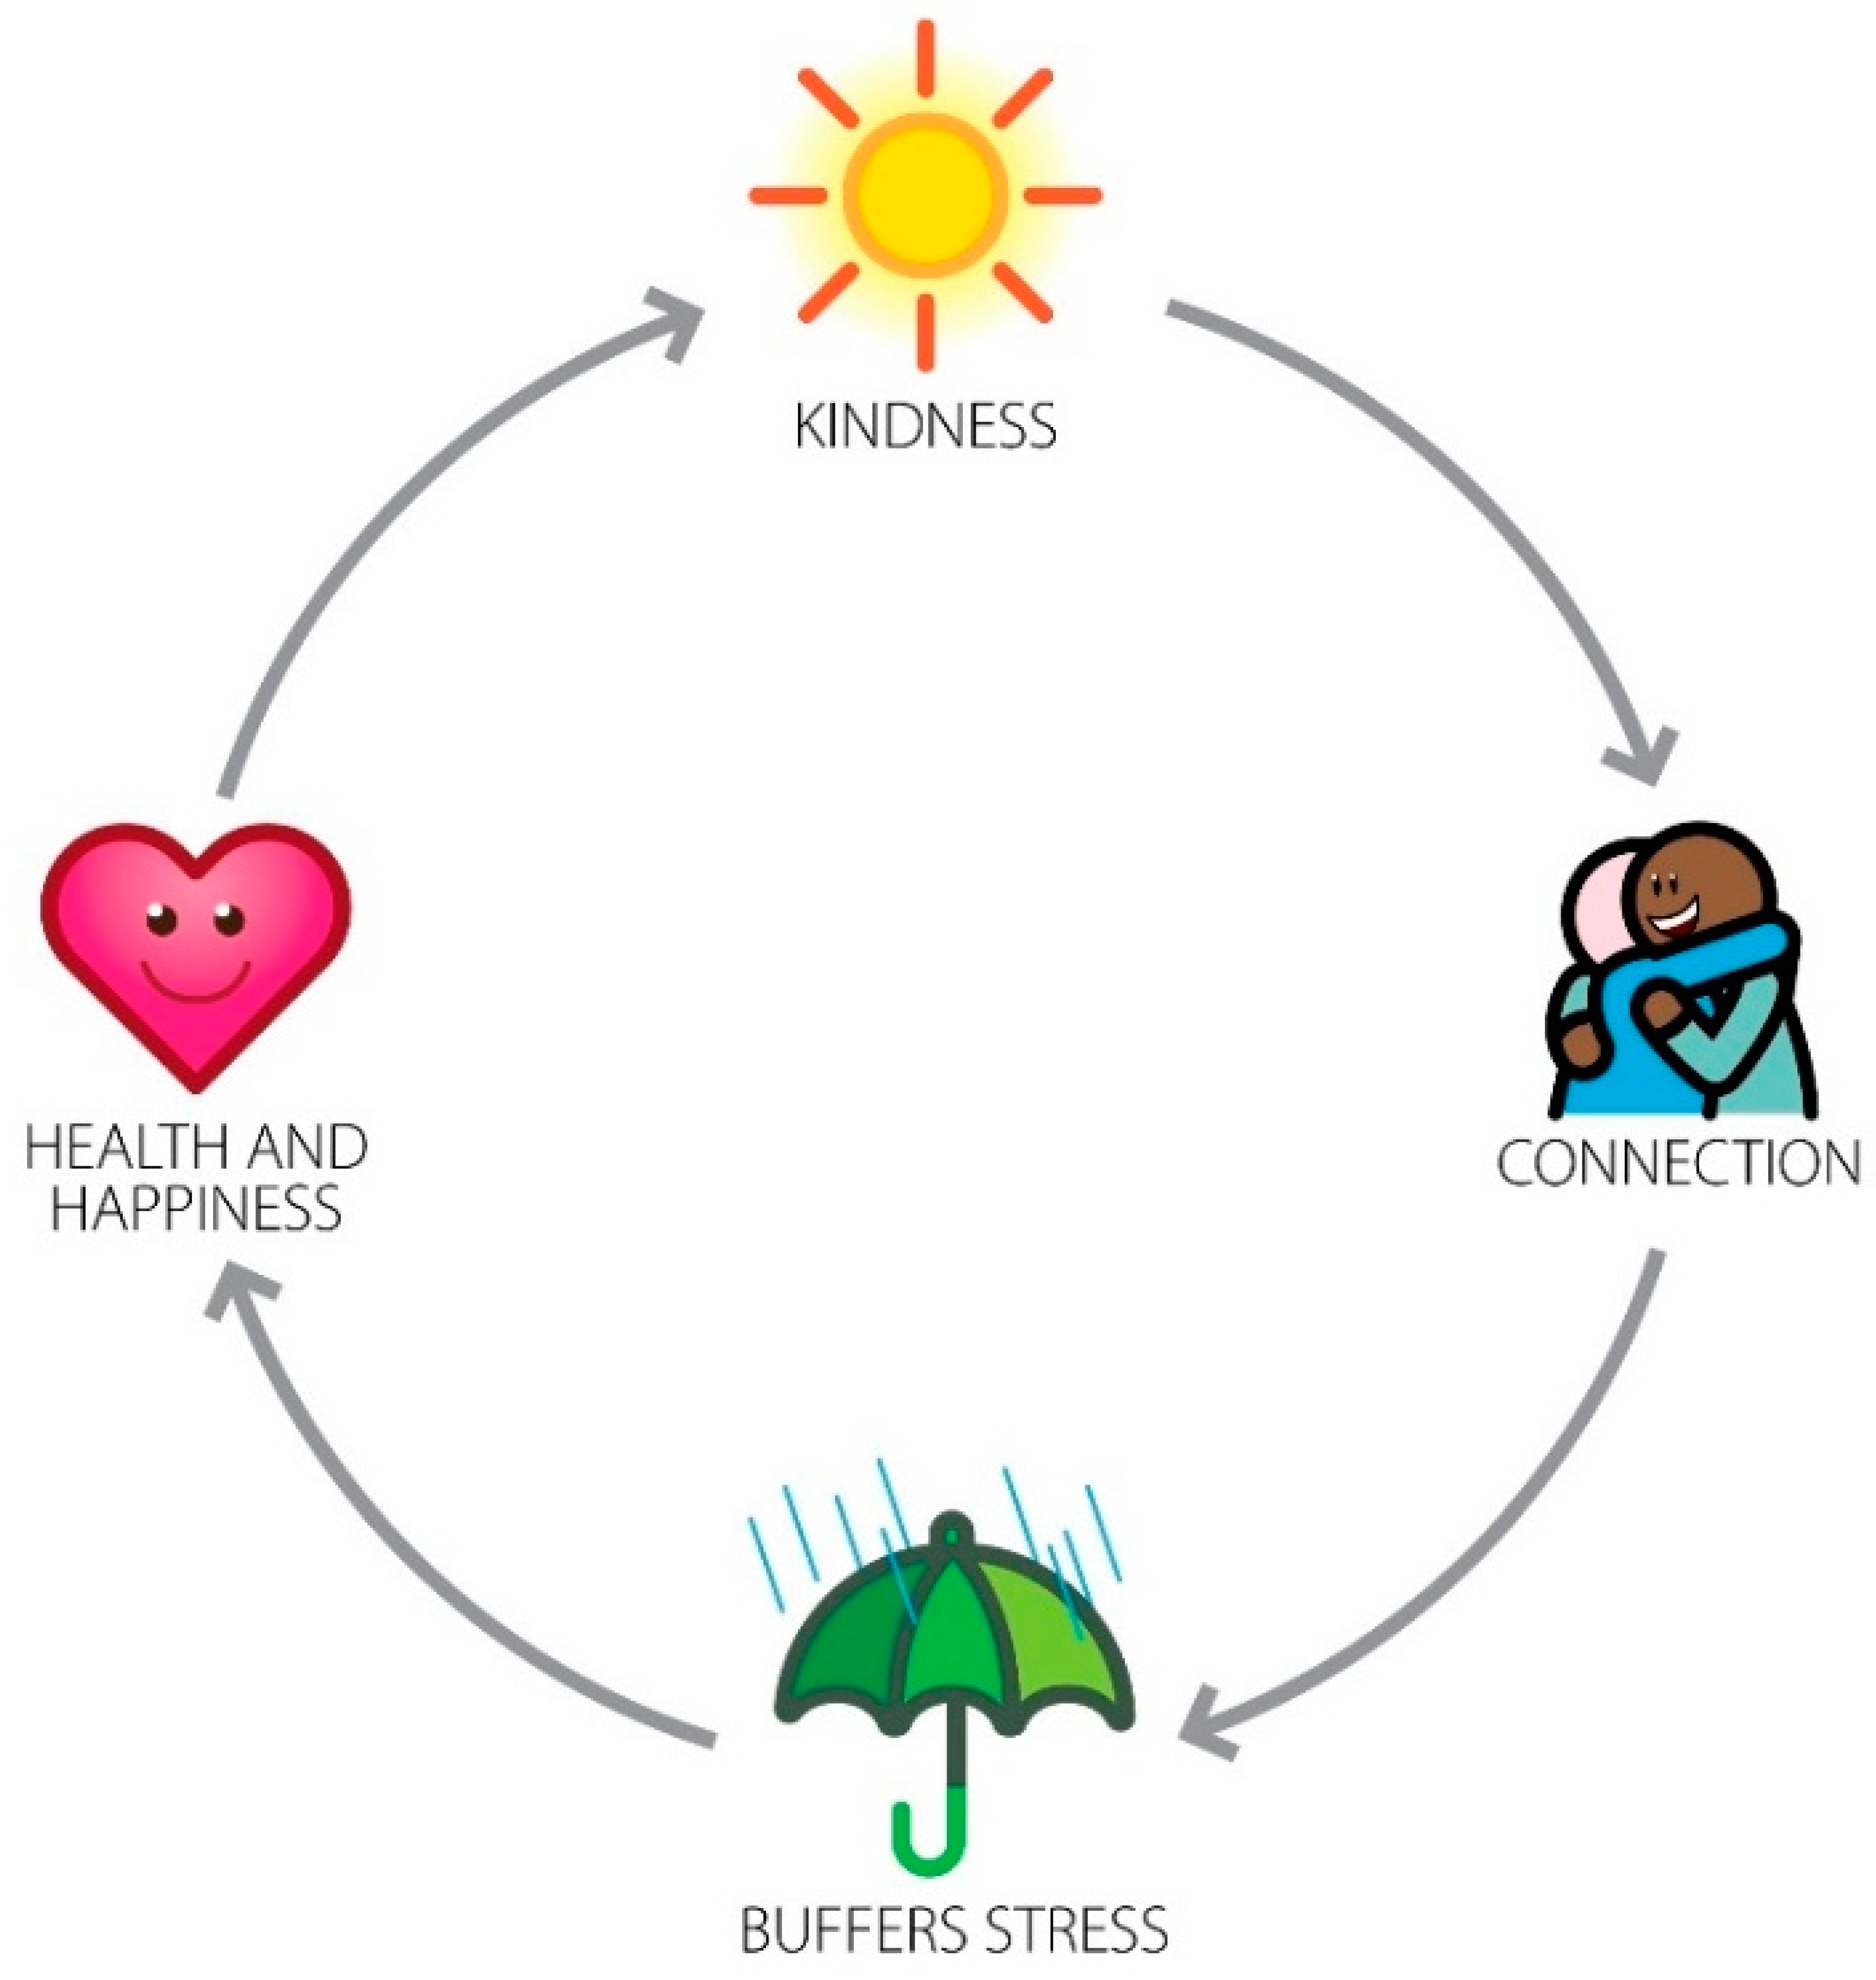
\includegraphics[width=\textwidth]{behavsci.png}
\captionof{figure}[LOF entry]{Kindness Cycle [1]} 
\vspace{5mm} %5mm vertical space

The social media sentiment analysis revealed a resonance between positive workplace experiences and online expressions of gratitude and satisfaction. Instances of companies embracing and publicizing their kindness initiatives saw an amplification of positive sentiment, both internally among employees and externally among potential stakeholders. This dual impact suggests that fostering continuous kindness not only enhances internal dynamics but also contributes to a positive organizational reputation.
\vspace{5mm} %5mm vertical space
\newline
Additionally, a subgroup analysis based on organizational size and industry type highlighted nuanced variations in the perceived impact of continuous kindness. Smaller organizations, for instance, exhibited a more immediate and pronounced positive response, emphasizing the potential for tailored kindness interventions based on organizational characteristics.

\section{Conclusion and Future Works}
In conclusion, the findings of this investigation underscore the transformative potential of continuous kindness in the workplace. Organizations that prioritize kindness are likely to witness not only improved employee satisfaction but also enhanced collaboration and overall organizational success [7]. Future research in this domain could delve deeper into specific interventions, assess their long-term impact, and explore the potential intersectionality of kindness with other organizational variables. Additionally, considering the evolving nature of work, examining the applicability of continuous kindness in virtual and hybrid work environments presents an intriguing avenue for further exploration.
\vspace{5mm} %5mm vertical space
\newline
In conclusion, the amalgamation of qualitative insights, case studies, survey data, and social media sentiment analysis paints a comprehensive picture of the transformative power of continuous kindness in the workplace. As organizations navigate the ever-evolving dynamics of the professional landscape, integrating kindness emerges not only as a moral imperative but as a strategic advantage for attracting and retaining talent.
\vspace{5mm} %5mm vertical space
\newline
Future research could delve into the cultural nuances that shape perceptions of kindness in diverse global workplaces. Furthermore, investigating the intersectionality of continuous kindness with other workplace initiatives, such as diversity and inclusion efforts, could provide a holistic understanding of organizational dynamics. Additionally, longitudinal studies tracking the sustained impact of kindness interventions over extended periods would contribute valuable insights into the long-term benefits of nurturing a kind workplace culture.

\pagebreak
\section{References}
1. Kindness Isn’t Just about Being Nice: The Value Proposition of Kindness as Viewed through the Lens of Incivility in the Healthcare Workplace (2023), David A. Fryburg, \url{https://www.mdpi.com/2076-328X/13/6/457}
\vspace{5mm} %5mm vertical space
\newline
2. THE IMPACT OF KINDNESS IN THE WORKPLACE (2008), DEBORAH LYNN KERR, \url{https://central.bac-lac.gc.ca/.item?id=MR55208&op=pdf&app=Library&is_thesis=1&oclc_number=738400260}
\vspace{5mm} %5mm vertical space
\newline
3. Bringing Self-Kindness Into the Workplace: Exploring the Mediating Role of Self-Compassion in the Associations Between Attachment and Organizational Outcomes (2019), Abira Reizer, \url{https://www.frontiersin.org/articles/10.3389/fpsyg.2019.01148/full}
\vspace{5mm} %5mm vertical space
\newline
4. Grace in the Workplace: A Process Model of its Impact (2022),  O'Connell, David, \url{ https://www.ingentaconnect.com/content/jmsr/rmsr20/2022/00000019/00000004/art00003}
\vspace{5mm} %5mm vertical space
\newline
5. A little thanks goes a long way: Explaining why gratitude expressions motivate prosocial behavior (2010), Grant Adam, \url{https://psycnet.apa.org/record/2010-09990-007}
\vspace{5mm} %5mm vertical space
\newline
6. Exploring Positive Relationships at Work (2007), Dutton and Ragins, \url{https://books.google.ca/books?hl=en&lr=&id=lBw3DwAAQBAJ&oi=fnd&pg=PT10&dq=Exploring+Positive+Relationships+at+Work&ots=EMToqlycF3&sig=7Pg2lHSzrkR7oI2Z0gDxukgE6DM#v=onepage&q=Exploring%20Positive%20Relationships%20at%20Work&f=false}
\vspace{5mm} %5mm vertical space
\newline
7. ChatGpt, Online AI Tool-
   Commands: Kindness at Workplace, Impact of Kindness at Work.
\end{document}